\subsection{Volume besturing}
\subsubsection{Voordeel voor de klant/ gebruiker van ...}
De volume besturing is puur gebruiksgemak voor de eindgebruiker. Er zit een display op de speakers waarop je alle nuttige informatie kan vinden van de speaker. Zo kan je bijvoorbeeld zien wat het volume is. Ook heb je de mogelijkheid om het volume te besturen via een knop maar ook via een app op je telefoon.
\subsubsection{Nadelen kosten van ...}
Door het volume op deze manier te besturen zal de prijs maar ook het verbruik van de speaker omhoog gaan. Dit gaat om ongeveer 60mA. 
\subsubsection{Hoe werkt ... en hoe ziet ... er uit}
De volume besturing gebruikt als brein een ESP8266 Wemos R1 D1 Mini. Deze controller heeft een WiFi module die als accespoint dient. Dit zorgt ervoor dat je kan inloggen op de module. Ook zijn er vier andere componenten aangesloten aan de controller. Ten eerste de rotary encoder, zo is het mogelijk om het volume te besturen via een fysieke knop maar ook via de app. Ten tweede heb je het display, hier kan je alle nuttige informatie op zien zoals het volume en de inloggegevens. Ten derde heb je de voltage regulator, dit omdat het ingangssignaal 9V is en ons circuit op 5V en 3.3V draait. Als laatst hebben we onze XDCP, of te wel de digitale potentiometer. Met behulp van deze potentiometer kunnen we het volume via de microcontroller besturen. Wat ons opviel is dat wij een ruis hadden rond 2.3 MHz, dit hebben we opgelost door een filter toe te voegen.

\begin{figure}[ht]
    \centering
    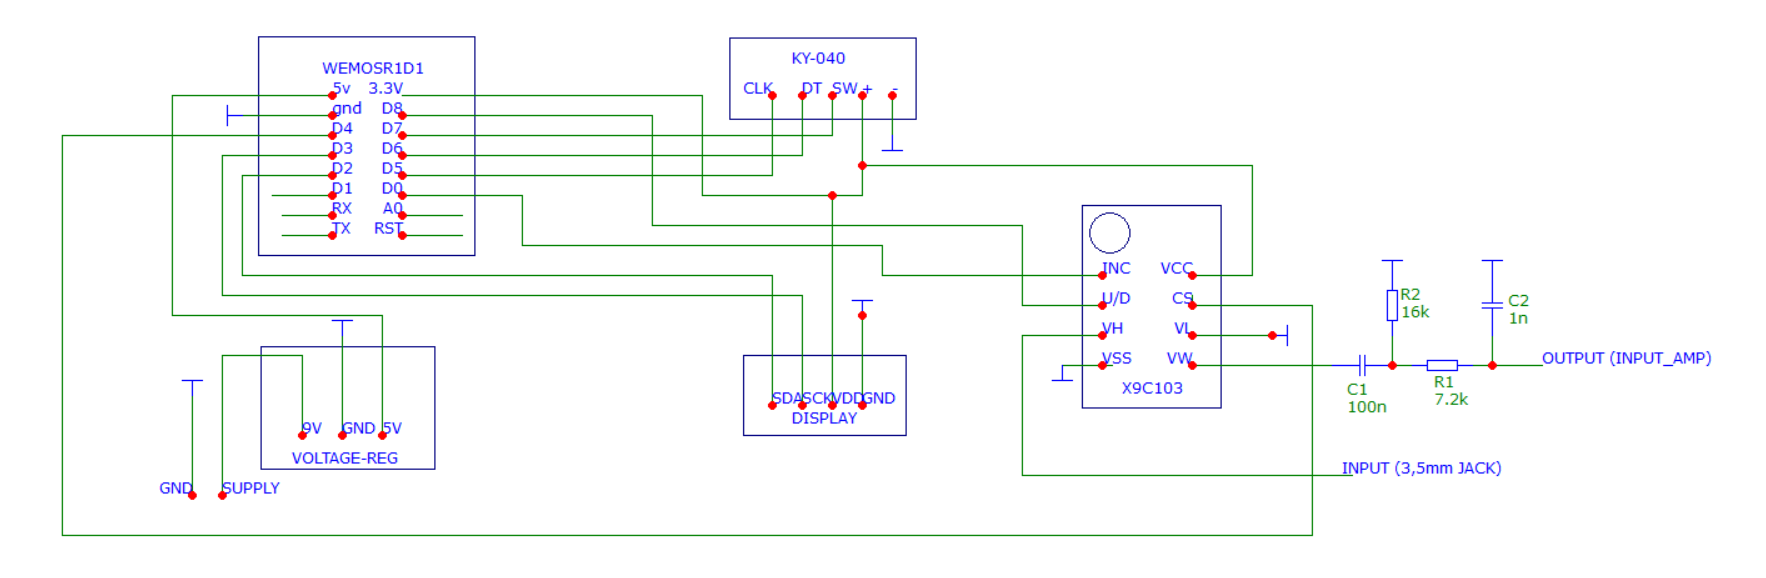
\includegraphics[width=0.90\textwidth]{IMG/004/Vol_ctr.png}
    \caption{Volume controller}
    \label{fig:Volume Controller}
\end{figure}